The scatter communication pattern reorganizes data and writes a single input data element to a single or multiple different output element(s) in memory.
This communication is used when a parallel tasks needs to write its result to a specific or multiple output elements.
It is similar to gather but instead it has a one-to-one/one-to-many correspondence between input and output(s) as seen in \autoref{fig:scatter}.
\begin{figure}[ht]
	\centering
	\fbox{
		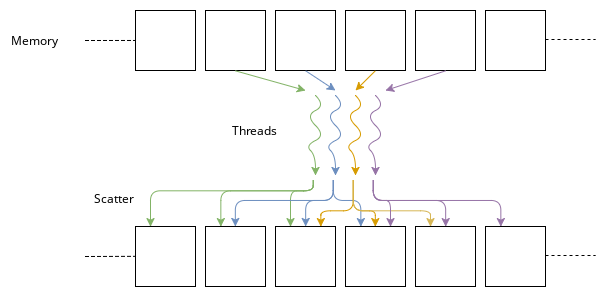
\includegraphics[width=0.6\textwidth]{figs/patterns/parallelscatter.png}
	}
	\caption{Scatter Pattern}
	\label{fig:scatter}
\end{figure}
\autoref{fig:scatter} suggests that there might be a synchronization issue which could lead to a \textit{data race}.
The problem is that several threads will very likely try to write to the same place in memory.
Say for instance that each thread has to increment a variable in memory which can be accessed by any thread.
This increment might not be correct because the variable might have been updated by another thread \textit{after} the variable has been read, which leads to data inconsistency.
This can be avoided by synchronizing threads or declaring the memory section as atomic.

The scatter pattern can for instance be used in combination with the gather pattern for representing sparse matrices which is more thoroughly described in section ?? bla. bla.